\section{Problem Formulation}\label{sec:pro}
In this section,
we first formally define the \textit{quality optimal sampling problem} (\prob{}) for large-scale trajectory data visualization in Section~\ref{sec:def},
and then show that it is NP-hard to solve the problem exactly in Section~\ref{sec:hard}.

\begin{figure}
	\centering
	\small
	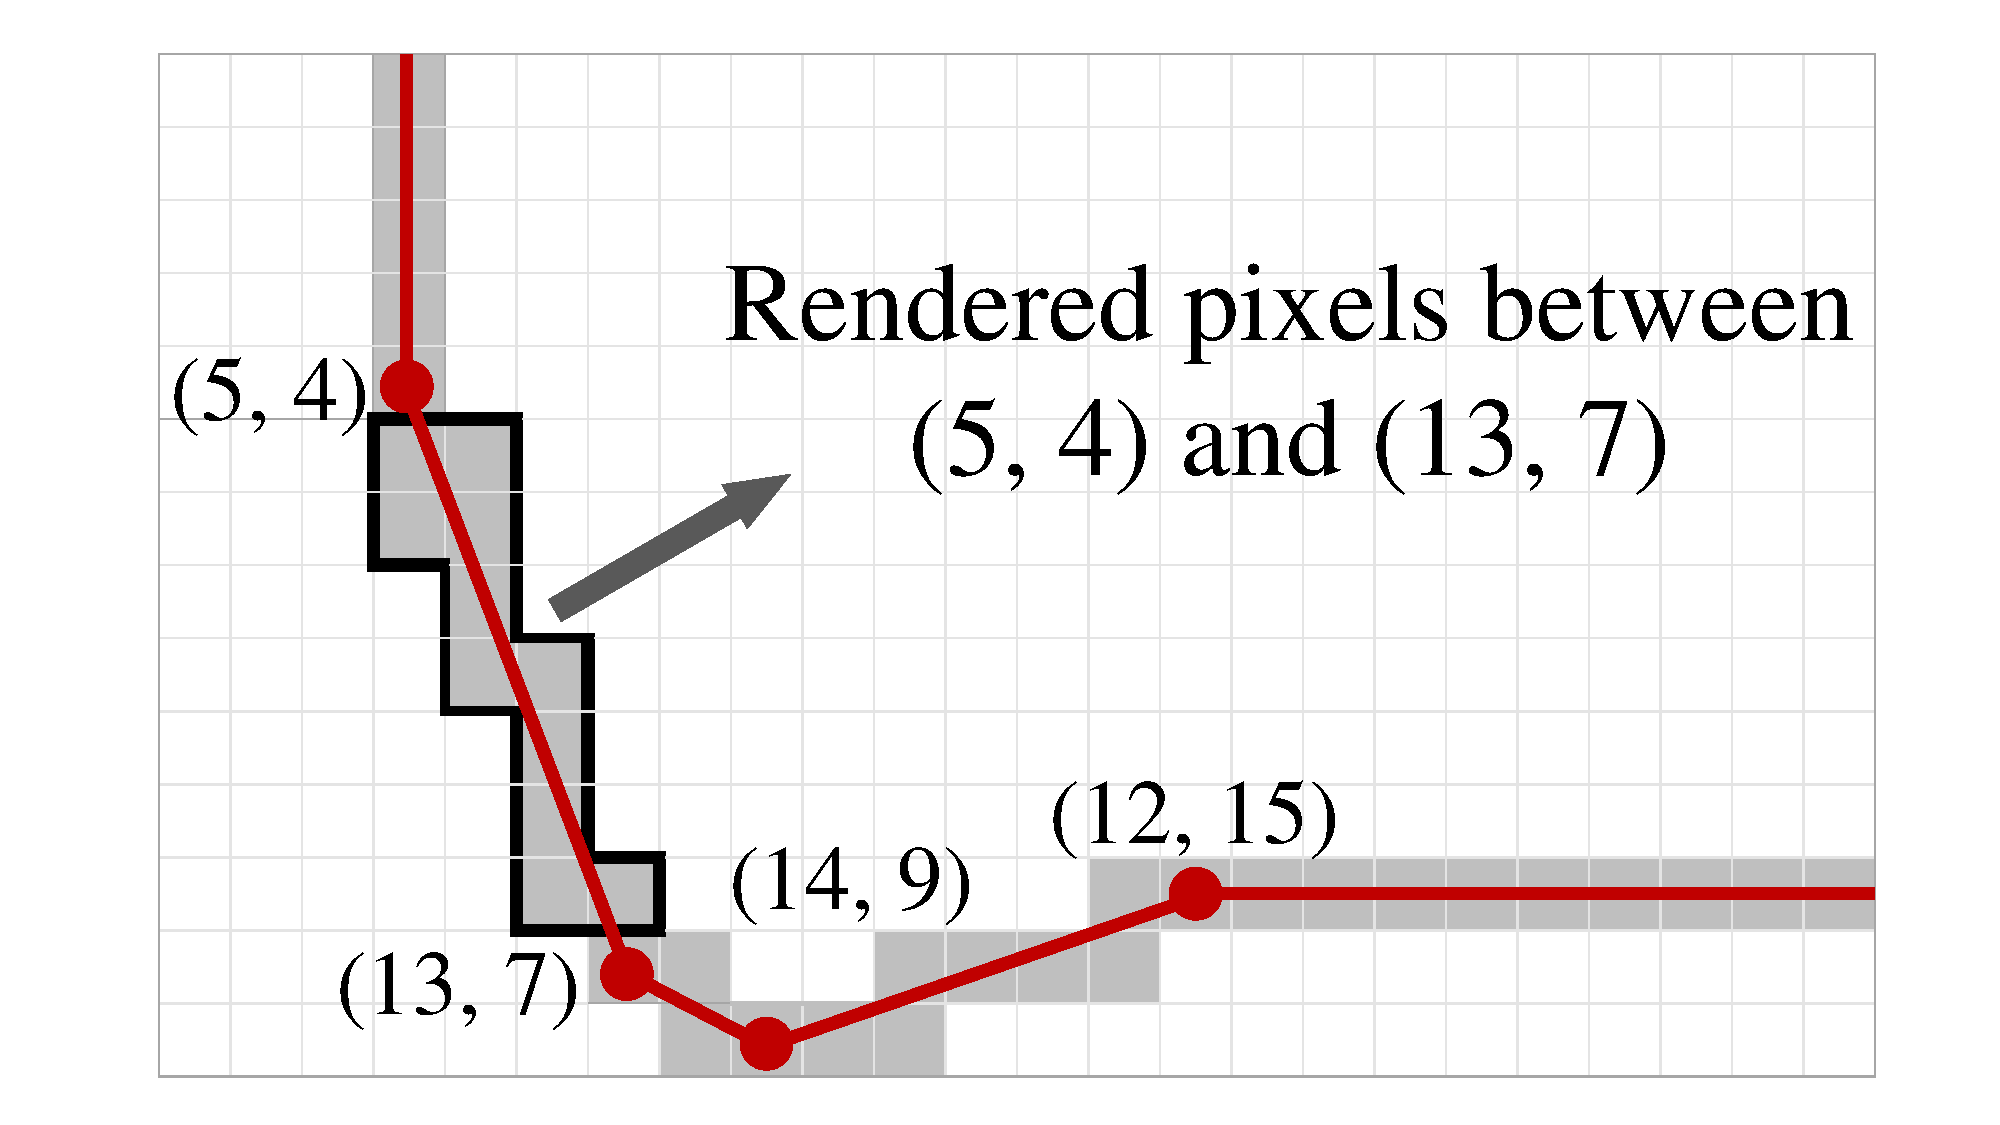
\includegraphics[width=0.5\columnwidth]{pictures/problemsolveing/RenderedPixels}  
    \trim
	\caption{Illustration of line-based trajectory visualization.} \label{fig:line}
    \trim \trim
\end{figure}


\subsection{Problem Definition}\label{sec:def}

We motivate our definition of the \textit{visualization quality function} by introducing how line-based trajectory visualization works.
As elaborated earlier, a trajectory contains a sequence of 2-dimensional locations.
Given an empty canvas (i.e., the screen of a displaying device) with pixels indexed by horizontal and vertical coordinates (i.e., $x$ and $y$), line-based trajectory visualization connects consecutive locations in each trajectory with polylines and marks the pixels passed by these polylines (with a color different from the background).
As shown in Figure~\ref{fig:line}(A), the result of line-based trajectory visualization can be regarded as a 2-dimensional array of boolean variables with 1 indicting that a pixel has been marked.
Alternatively, we can treat a visualization result as a set $\mathcal{S}=\{(x_i, y_i)\}_{i=1}^{n}$ that contains all marked pixels.
This observation leads to the following definition of visualization quality function
\begin{equation}\label{eqref:loss}
\QQ(\mathcal{S}, \mathcal{S}')=\frac{|\mathcal{S} \cap \mathcal{S}'|}{|\mathcal{S}|},
\end{equation}
in which $|.|$ measures the cardinality of a set, $\mathcal{S}$ is the visualization result of the entire trajectory dataset $\mathcal{T}$ while $ \mathcal{S}'$ is the visualization result of some trajectories sampled from $\mathcal{T}$.
As $\mathcal{S}'\subseteq \mathcal{S}$, $\QQ(\mathcal{S}, \mathcal{S}')$ essentially measures the ratio of the pixels in the ground-truth visualization $\mathcal{S}$ that are marked in the approximate visualization $\mathcal{S}'$.
%\footnote{For more general cases with $\mathcal{V}'\not\subset \mathcal{V}$, the quality function can be defined as $\mathsf{q}(\mathcal{V}, \mathcal{V}')\!=\!\frac{|\mathcal{V}-\mathcal{V}'|}{|\mathcal{V}|}$, in which set $\mathcal{V}^\star\!=\!\mathcal{V}-\mathcal{V}'$ contains all distinct elements between $\mathcal{V}$ and $\mathcal{V}'$.}.
This definition matches human visual perception and the approximate visualization $\mathcal{S}'$ will look similar to $\mathcal{S}$ if $\QQ(\mathcal{S}, \mathcal{S}')$ is large.
Sampling reduces the number of trajectories and location points to process, and thus shortens the visualization time.
With the quality function, we define the quality optimal sampling problem as follows.

\begin{problem}[Quality Optimal Sampling Problem, \prob{}]\label{prob:def}
Let the entire trajectory dataset be $\mathcal{T}$ and a sample set that contains some trajectories from $\mathcal{T}$ be $\mathcal{R}$.
Using $\VV(\mathcal{U})$ to denote the visualization result set derived from a trajectory set $\mathcal{U}$, with a sampling rate $\alpha$,
the quality optimal sampling problem finds a set $\mathcal{R}$ that satisfies
	\begin{equation}\label{eq:opp}
	\max_{\mathcal{R} \subseteq \mathcal{T}, |\mathcal{R}| = \lceil \alpha |\mathcal{T}| \rceil} \QQ(\VV(\mathcal{T}), \VV(\mathcal{R}))=\frac{|\VV(\mathcal{T}) \cap \VV(\mathcal{R})|}{|\VV(\mathcal{T})|}.
	\end{equation}
\end{problem}
Note that we are sampling \textit{complete trajectories} instead of \textit{individual locations} in \prob{} such that the lines and orientations in the trajectories are persevered.

Intuitively, given a visualization quality threshold $\tau$, the \prob{} problem can be transformed to find the sampled trajectory set $\mathcal{R}$ with the smallest $\alpha$,
under which provides the quality requirement holds, i.e, $\QQ(\VV(\mathcal{T}), \VV(\mathcal{R})) \!\ge\! \tau$.




\subsection{Hardness Analysis}\label{sec:hard}
We use $t_i\! \in \! \mathcal{T}$ to denote a trajectory in the dataset.
According to the working mechanism of line-based trajectory visualization, $t_i$ corresponds to a set of marked pixels on the canvas in the ground-truth visualization $\VV(\mathcal{T})$ and we also use $t_i$ to denote this set of pixels.
Thus, we have $\VV(\mathcal{T}) = \cup_{t_i \in \mathcal{T}} t_i$ and $\VV(\mathcal{R}) = \cup_{t_i \in \mathcal{R}} t_i$.
We can transform Problem~\ref{prob:def} as follows:

\begin{align}\label{eqn:obj2}
& \max_{\oR \subseteq \D, |\oR| = \lceil \alpha |\mathcal{T}| \rceil}  \frac{|\VV(\mathcal{T}) \cap \VV(\mathcal{R})|}{|\VV(\mathcal{T})|} \\ \nonumber
& \Leftrightarrow \max_{\oR \subseteq \D, |\oR| = \lceil \alpha |\mathcal{T}| \rceil}   |\VV(\oR)|   %\\ \nonumber
 \Leftrightarrow \max_{\oR \subseteq \D, |\oR| = \lceil \alpha |\mathcal{T}| \rceil} | \cup_{t_i \in \oR} t_i |.
\end{align}

%\begin{align}\label{eqn:obj5} \nonumber
%	\min_{\oR \subseteq \D, |\oR| = \alpha |\D|}  \frac{|\V(\D) - \V(\oR)|}{|\V(\D)|}  & \Leftrightarrow \min_{\oR \subseteq \D, |\oR| = \alpha |\D|}   - |\V(\oR)| \\ \nonumber
%	\Leftrightarrow \max_{\oR \subseteq \D, |\oR| = \alpha |\D|}  |\V(\oR)| &  \Leftrightarrow \max_{\oR \subseteq \D, |\oR| = \alpha |\D|} | \cup_{t_i \in \oR} t_i |
%\end{align}

The transformations use the fact that $\VV(\mathcal{R}) \!\subseteq \! \VV(\mathcal{T})$ as $\mathcal{R}\! \subseteq \! \mathcal{T}$, and the ground-truth marked point set $\VV(\mathcal{T})$ has constant cardinality.
The last line shows that \prob{} is equivalent to the famous set cover maximization problem\footnote{\url{https://en.wikipedia.org/wiki/Maximum_coverage_problem}}.
Specifically, given an integer $k$, and a collection of sets $\D = \{t_1, t_2, \cdots, t_n \}$,
set cover maximization finds a subset $\oR \subset \D$ such that $|\oR| = k$ and the number of covered elements $|\cup_{t_i \in \oR} t_i|$ is maximized.
The set cover maximization problem is well-known to be NP-hard~\cite{algorithms}.
For sampling-based methods, the visualization quality is determined by the sample set $\mathcal{R}$,
and thus we use $\QQ(\mathcal{R})$ to denote $\QQ(\VV(\mathcal{T}), \VV(\mathcal{R}))$ for conciseness.




%It is equivalent to select sized-$k$ trajectory set $\oR$ from $\D$ which $\cup_{\oR_i \in \oR} \oR_i$ is maximized.
%It is a NP-hard problem as we proved in Lemma~\ref{lem:np}.

%\begin{lemma}[NP hard]~\label{lem:np}
%Given a trajectory dataset $\D$ and an integer $k$,
%The sampling-based trajectory visualization problem (see Problem~\ref{prob:def}) is NP-hard.
%\end{lemma}

%We omit the proof of Lemma~\ref{lem:np} as it is a typical set cover maximization problem\footnote{\url{https://en.wikipedia.org/wiki/Maximum_coverage_problem}}, which is a well-known NP-hard problem in literature.

%------------comments by Bo-------------------
%As we analyzed in Section~\ref{sec:intro}, the large-scale (e.g., hundreds of millions GPS points) line-based trajectory visualization problem is very challenging due to the large data size and limited rendering capability of graphics devices.
%To make matters worse, the visualization result of large-scale trajectory dataset suffers visual clutter seriously.
%In this work, we focus on how to visualize large-scale trajectory dataset efficiently and effectively.
%In particular, our objective is to devise a visual quality guaranteed sampling method for large trajectory data visualization.
%The major challenges to achieve this goal are:
%(i) how to define visual quality theoretically? (ii) how to guarantee the visual quality of the sampling-based visualization result?
